\documentclass[aspectratio=169,11pt]{beamer}
\usetheme{Madrid}
\usecolortheme{default}
\usepackage{amsmath,amssymb,bm,mathtools}
\usepackage{graphicx}
\usepackage{booktabs}
\usepackage{tikz}
\usepackage{array}
\usepackage{ragged2e}
\setbeamertemplate{navigation symbols}{}
\setbeamertemplate{footline}[frame number]
\setbeamercolor{title}{fg=red!75!black}
\setbeamercolor{frametitle}{fg=red!75!black}
\setbeamertemplate{itemize item}{\color{red!75!black}$\blacktriangleright$}
\setbeamersize{text margin left=7mm,text margin right=7mm}
\title{Composite Materials}
\author{Gajavada Sanjeevkumar}
\date{06 November 2026}
\newcommand{\sym}{\text{\scriptsize Symmetry}}
\newcommand{\mat}[1]{\begin{bmatrix}#1\end{bmatrix}}
\newcommand{\vect}[1]{\left\{#1\right\}}
\newcommand{\R}{\mathbb{R}}
\begin{document}

% 1
\begin{frame}{What are composite materials?}
\small
Two or more materials from the first three categories (metals, polymers, ceramics)
combined on a macroscopic scale to form a useful third material.
\vspace{2mm}
\textcolor{red!75!black}{\textbf{Advantages:}} Some properties that can be improved by forming a composite material
(should be different from those of the constituents):
\begin{columns}[T]
\column{.48\textwidth}
\begin{itemize}
\item Strength \item Stiffness \item Corrosion resistance
\item Wear resistance \item Fatigue life \item Thermal conductivity
\end{itemize}
\column{.48\textwidth}
\begin{itemize}
\item Thermal insulation \item Attractiveness \item Weight
\item Acoustical insulation \item Temperature-dependent behavior
\end{itemize}
\end{columns}
\textcolor{red!75!black}{\textbf{Note:}} Not all these properties improve at the same time.
\end{frame}

% 2
\begin{frame}{Materials/Phases}
\begin{itemize}
\item One phase is discontinuous, stiffer and stronger, and is called the
\textbf{reinforcement}.
\item The other phase is continuous, less stiff and weaker, and is called the
\textbf{matrix}.
\end{itemize}
\begin{center}
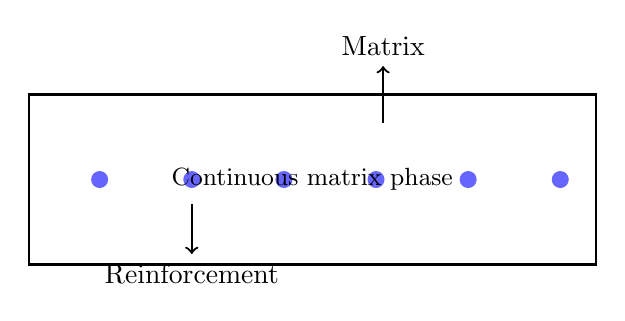
\begin{tikzpicture}[scale=.9]
\draw[thick] (0,0) rectangle (8,2.4);
\foreach \x in {1,2.3,3.6,4.9,6.2,7.5}
  \fill[blue!60] (\x,1.2) circle (.12);
\draw[->,thick] (2.3,.85)--(2.3,.15) node[below]{Reinforcement};
\draw[->,thick] (5,2.0)--(5,2.8) node[above]{Matrix};
\node at (4,1.2) {\small Continuous matrix phase};
\end{tikzpicture}
\end{center}
\end{frame}

% 3
\begin{frame}{Composite Materials}
\begin{center}
\includegraphics[width=.88\linewidth,height=.72\textheight,keepaspectratio]{figures/s03_img01.png}
\end{center}
\end{frame}

% 4
\begin{frame}{Composite Materials}
\small
\textcolor{red!75!black}{\textbf{Fibrous Composite:}}
\begin{itemize}
\item Wood (spirally wound cellulose fibres + lignin)
\item Bone (organic collagen fibres + small inorganic crystals, water and fats; femur)
\item Plywood
\item Fibre glass (glass fibre + polyester/epoxy/phenolic matrix)
\item Long fibrous composite (glass/Kevlar/carbon/nylon fibres + matrix)
\end{itemize}
\textcolor{red!75!black}{\textbf{Granular / Particulate Composite:}}
\begin{itemize}
\item Granite (quartz, feldspar, mica + granular phase)
\item Concrete (cement, sand and small pebbles)
\item Cermets (ceramics + metals)
\end{itemize}
\end{frame}

% 5
\begin{frame}{Composite Materials}
\begin{center}
\includegraphics[width=.92\linewidth,height=.76\textheight,keepaspectratio]{figures/s05_img01.png}
\end{center}
\end{frame}

% 6
\begin{frame}{Applications}
\small
\textcolor{red!75!black}{\textbf{Automotive Sector}}
\begin{itemize}
\item Lightweight, strong, wear- and rust-resistant, aesthetic appearance.
\item Car body, brake pads, drive shafts, fuel tank, bonnet, spoilers, leaf springs, etc.
\end{itemize}
\textcolor{red!75!black}{\textbf{Aerospace Sector}}
\begin{itemize}
\item Lightweight, strong, temperature- and wear-resistant; smart structures.
\item Aircraft: nose, doors, wings, spoilers, cowlings, fin tips, flaps, stabilizers.
\item Rockets and missiles: nose, body, pressure and fuel tanks.
\item Satellites: frames, structural parts, antenna (smart materials).
\end{itemize}
\end{frame}

% 7
\begin{frame}{Applications}
\small
\textcolor{red!75!black}{\textbf{Sports Sector}}
\begin{itemize}
\item Lightweight, strong, aesthetic and high damping.
\item Tennis/badminton racquets, hockey, golf, diving boards, helmets, etc.
\end{itemize}
\textcolor{red!75!black}{\textbf{Transportation and Infrastructure Sector}}
\begin{itemize}\item Lightweight, strong, tough and high damping.\end{itemize}
\textcolor{red!75!black}{\textbf{Biomedical Sector}}
\begin{itemize}\item Consumer goods, agricultural equipment, healthcare industry and chemical industry.\end{itemize}
\end{frame}

% 8
\begin{frame}{Classification}
\begin{center}
\includegraphics[width=.94\linewidth,height=.76\textheight,keepaspectratio]{figures/s08_img01.jpg}
\end{center}
\end{frame}

% 9
\begin{frame}{Classification}
\begin{center}
\includegraphics[width=.94\linewidth,height=.76\textheight,keepaspectratio]{figures/s09_img01.png}
\end{center}
\end{frame}

% 10
\begin{frame}{Limitations}
\small
\begin{itemize}
\item \textbf{Anisotropy:} analysis is more complicated and difficult; it takes more time.
\item \textbf{Non-homogeneous.}
\item \textbf{Costly:} for example, fibre glass requires glass-fibre reinforcement and polyester matrix.
\item \textbf{Difficult to fabricate.}
\item \textbf{Sensitive to temperature:} thermal conductivities of matrix and fibres are different.
\item \textbf{Sensitive to moisture:} residual hygroscopic stresses.
\end{itemize}
\end{frame}

% 11
\begin{frame}{Micromechanics of Lamina}
\begin{columns}[T]
\column{.62\textwidth}
\begin{itemize}
\item Generalized Hooke's law
\item Anisotropic elasticity
\item Constitutive relations
\item Planes of material-property symmetry
\item Triclinic, monoclinic, orthotropic and isotropic materials
\item Engineering constants for orthotropic materials
\item Lamina is an anisotropic material
\end{itemize}
\column{.35\textwidth}
\begin{center}
\includegraphics[width=\linewidth,height=.55\textheight,keepaspectratio]{figures/s11_img01.jpg}
\end{center}
\end{columns}
\end{frame}

% 12
\begin{frame}{Generalized Hooke's Law in 3D}
\small
For a general anisotropic, linearly elastic material:
\[
\begin{Bmatrix}\sigma_{xx}\\\sigma_{yy}\\\sigma_{zz}\\\tau_{yz}\\\tau_{xz}\\\tau_{xy}\end{Bmatrix}
=
\begin{bmatrix}
C_{11}&C_{12}&C_{13}&C_{14}&C_{15}&C_{16}\\
\sym&C_{22}&C_{23}&C_{24}&C_{25}&C_{26}\\
\sym&\sym&C_{33}&C_{34}&C_{35}&C_{36}\\
\sym&\sym&\sym&C_{44}&C_{45}&C_{46}\\
\sym&\sym&\sym&\sym&C_{55}&C_{56}\\
\sym&\sym&\sym&\sym&\sym&C_{66}
\end{bmatrix}
\begin{Bmatrix}\epsilon_{xx}\\\epsilon_{yy}\\\epsilon_{zz}\\\gamma_{yz}\\\gamma_{xz}\\\gamma_{xy}\end{Bmatrix}
\]
\vspace{-1mm}
\[
\{\boldsymbol{\sigma}\}=[C]\{\boldsymbol{\epsilon}\},
\qquad
\{\boldsymbol{\epsilon}\}=[S]\{\boldsymbol{\sigma}\},\quad [S]=[C]^{-1}.
\]
\end{frame}

% 13
\begin{frame}{Generalized Hooke's Law in 3D}
\small
The compliance form of the generalized Hooke's law is
\[
\begin{Bmatrix}\epsilon_{xx}\\\epsilon_{yy}\\\epsilon_{zz}\\\gamma_{yz}\\\gamma_{xz}\\\gamma_{xy}\end{Bmatrix}
=
\begin{bmatrix}
S_{11}&S_{12}&S_{13}&S_{14}&S_{15}&S_{16}\\
\sym&S_{22}&S_{23}&S_{24}&S_{25}&S_{26}\\
\sym&\sym&S_{33}&S_{34}&S_{35}&S_{36}\\
\sym&\sym&\sym&S_{44}&S_{45}&S_{46}\\
\sym&\sym&\sym&\sym&S_{55}&S_{56}\\
\sym&\sym&\sym&\sym&\sym&S_{66}
\end{bmatrix}
\begin{Bmatrix}\sigma_{xx}\\\sigma_{yy}\\\sigma_{zz}\\\tau_{yz}\\\tau_{xz}\\\tau_{xy}\end{Bmatrix}.
\]
\end{frame}

% 14
\begin{frame}{Generalized Hooke's Law in 3D}
\small
Due to equality of cross shear (from moment equilibrium in the absence of body
moments),
\[
\sigma_{ij}=\sigma_{ji},\qquad
\epsilon_{ij}=\epsilon_{ji},\quad i\ne j.
\]
Thus the stress and strain tensors are symmetric:
\[
[\sigma]=
\begin{bmatrix}
\sigma_{xx}&\tau_{xy}&\tau_{xz}\\
\sym&\sigma_{yy}&\tau_{yz}\\
\sym&\sym&\sigma_{zz}
\end{bmatrix},
\qquad
[\epsilon]=
\begin{bmatrix}
\epsilon_{xx}&\epsilon_{xy}&\epsilon_{xz}\\
\sym&\epsilon_{yy}&\epsilon_{yz}\\
\sym&\sym&\epsilon_{zz}
\end{bmatrix}.
\]
\end{frame}

% 15
\begin{frame}{Anisotropic Elasticity}
\small
From energy considerations, for a linearly elastic material the stiffness and
compliance matrices are also symmetric:
\[
C_{ij}=C_{ji},\qquad S_{ij}=S_{ji}.
\]
\[
[C]=
\begin{bmatrix}
C_{11}&C_{12}&C_{13}&C_{14}&C_{15}&C_{16}\\
\sym&C_{22}&C_{23}&C_{24}&C_{25}&C_{26}\\
\sym&\sym&C_{33}&C_{34}&C_{35}&C_{36}\\
\sym&\sym&\sym&C_{44}&C_{45}&C_{46}\\
\sym&\sym&\sym&\sym&C_{55}&C_{56}\\
\sym&\sym&\sym&\sym&\sym&C_{66}
\end{bmatrix}.
\]
\end{frame}

% 16
\begin{frame}{Anisotropic Elasticity}
\begin{center}
\Large Stiffness and compliance matrices have 21 independent elastic constants.
\end{center}
\[
N=\frac{6(6+1)}{2}=21.
\]
The symmetry of the constitutive matrices reduces the 36 entries to 21
independent constants.
\end{frame}

% 17
\begin{frame}{Planes of Material-Property Symmetry -- Monoclinic Materials}
\small
\begin{itemize}
\item A plane of material-property symmetry is a plane about which the material
properties remain unchanged under a 180$^\circ$ rotation.
\item For example, the $X$--$Y$ plane is a plane of material-property symmetry.
\end{itemize}
\begin{center}
\includegraphics[width=.5\linewidth,height=.42\textheight,keepaspectratio]{figures/s17_img01.png}
\end{center}
\end{frame}

% 18
\begin{frame}{Planes of Material-Property Symmetry -- Monoclinic Materials}
\small
Since the $Z$-plane is the plane of material-property symmetry, the stiffness
matrix remains the same in both cases. Hence stresses and strains in both
coordinate descriptions are related by the same stiffness matrix.
\[
[C]=
\begin{bmatrix}
C_{11}&C_{12}&C_{13}&C_{14}&C_{15}&C_{16}\\
\sym&C_{22}&C_{23}&C_{24}&C_{25}&C_{26}\\
\sym&\sym&C_{33}&C_{34}&C_{35}&C_{36}\\
\sym&\sym&\sym&C_{44}&C_{45}&C_{46}\\
\sym&\sym&\sym&\sym&C_{55}&C_{56}\\
\sym&\sym&\sym&\sym&\sym&C_{66}
\end{bmatrix}.
\]
\end{frame}

% 19
\begin{frame}{Planes of Material-Property Symmetry -- Monoclinic Materials}
\small
Using stress and strain transformations about the rotated axes:
\[
\{\sigma'\}=[T_\sigma]\{\sigma\},\qquad
\{\epsilon'\}=[T_\epsilon]\{\epsilon\}.
\]
For a 180$^\circ$ rotation about the symmetry-plane normal, the transformed
constitutive relation must represent the same material:
\[
[C]'=[T_\sigma][C][T_\epsilon]^{-1}=[C].
\]
\end{frame}

% 20
\begin{frame}{Planes of Material-Property Symmetry -- Monoclinic Materials}
\small
For a monoclinic material with one plane of material-property symmetry, the
stiffness matrix has the form (Voigt order: $11,22,33,23,13,12$):
\[
[C]=
\begin{bmatrix}
C_{11}&C_{12}&C_{13}&0&C_{15}&0\\
\sym&C_{22}&C_{23}&0&C_{25}&0\\
\sym&\sym&C_{33}&0&C_{35}&0\\
\sym&\sym&\sym&C_{44}&0&C_{46}\\
\sym&\sym&\sym&\sym&C_{55}&0\\
\sym&\sym&\sym&\sym&\sym&C_{66}
\end{bmatrix}.
\]
\begin{itemize}
\item The stiffness matrix consists of only 13 independent elastic constants.
\item An example of a monoclinic material is feldspar.
\end{itemize}
\end{frame}

% 21
\begin{frame}{Planes of Material-Property Symmetry -- Orthotropic Materials}
\small
If, in addition to one plane of material-property symmetry, there is another
perpendicular plane, then a third mutually perpendicular plane is also a plane
of material-property symmetry.
\vspace{2mm}
If the $Y$-plane is also a symmetry plane, inversion of the $Y$-axis gives
\[
X'=X,\qquad Y'=-Y,\qquad Z'=Z.
\]
The stiffness matrix remains unchanged under this coordinate inversion.
\end{frame}

% 22
\begin{frame}{Planes of Material-Property Symmetry -- Orthotropic Materials}
\small
The direction-cosine matrix for the coordinate transformation from
$(X,Y,Z)$ to $(X',Y',Z')$ is
\[
[a]=
\begin{bmatrix}
1&0&0\\
0&-1&0\\
0&0&1
\end{bmatrix}.
\]
Using stress and strain transformations about the rotated axes:
\[
\{\sigma'\}=[T_\sigma]\{\sigma\},\qquad
\{\epsilon'\}=[T_\epsilon]\{\epsilon\}.
\]
\end{frame}

% 23
\begin{frame}{Planes of Material-Property Symmetry -- Orthotropic Materials}
\small
For three mutually perpendicular planes of material-property symmetry, the
stiffness matrix is
\[
[C]=
\begin{bmatrix}
C_{11}&C_{12}&C_{13}&0&0&0\\
\sym&C_{22}&C_{23}&0&0&0\\
\sym&\sym&C_{33}&0&0&0\\
\sym&\sym&\sym&C_{44}&0&0\\
\sym&\sym&\sym&\sym&C_{55}&0\\
\sym&\sym&\sym&\sym&\sym&C_{66}
\end{bmatrix}.
\]
\begin{itemize}
\item Twelve elements become zero; only 9 independent elastic constants are required.
\item Examples: unidirectional lamina and rolled steel.
\end{itemize}
\end{frame}

% 24
\begin{frame}{Planes of Material-Property Symmetry -- Transversely Isotropic Materials}
\small
\begin{itemize}
\item Transversely isotropic materials are orthotropic materials with one
transverse plane of symmetry in which properties are independent of direction
(a plane of isotropy).
\item The 1-axis remains unchanged, while the 2--3 plane is rotated by an angle
$\theta$.
\end{itemize}
\[
[a]=
\begin{bmatrix}
1&0&0\\
0&\cos\theta&\sin\theta\\
0&-\sin\theta&\cos\theta
\end{bmatrix}.
\]
\end{frame}

% 25
\begin{frame}{Planes of Material-Property Symmetry -- Transversely Isotropic Materials}
\small
For transverse isotropy, rotation by any angle $\theta$ in the isotropic plane
must leave the constitutive law unchanged:
\[
[C]'=[C],\qquad [C]'=[T_\sigma][C][T_\epsilon]^{-1}.
\]
\begin{itemize}
\item Five independent elastic constants characterize a transversely isotropic material.
\item Example: UD lamina where fibres are arranged in a square array.
\end{itemize}
\end{frame}

% 26
\begin{frame}{Planes of Material-Property Symmetry -- Isotropic Materials}
\small
\begin{itemize}
\item Isotropic materials are those in which all planes are planes of material-property symmetry.
\item Two independent elastic constants are required to characterize isotropic materials.
\end{itemize}
\[
G=\frac{E}{2(1+\nu)},\qquad
\lambda=\frac{E\nu}{(1+\nu)(1-2\nu)}.
\]
\end{frame}

% 27
\begin{frame}{Generalized Hooke's Law in 3D (Isotropic)}
\small
The isotropic stiffness relation is
\[
\{\sigma\}=[C]\{\epsilon\},\qquad
[C]=
\begin{bmatrix}
\lambda+2G&\lambda&\lambda&0&0&0\\
\sym&\lambda+2G&\lambda&0&0&0\\
\sym&\sym&\lambda+2G&0&0&0\\
\sym&\sym&\sym&G&0&0\\
\sym&\sym&\sym&\sym&G&0\\
\sym&\sym&\sym&\sym&\sym&G
\end{bmatrix}.
\]
\end{frame}

% 28
\begin{frame}{Generalized Hooke's Law in 3D (Isotropic)}
\small
In terms of Young's modulus $E$ and Poisson's ratio $\nu$:
\[
\{\epsilon\}=[S]\{\sigma\},
\quad
[S]=\frac{1}{E}
\begin{bmatrix}
1&-\nu&-\nu&0&0&0\\
\sym&1&-\nu&0&0&0\\
\sym&\sym&1&0&0&0\\
\sym&\sym&\sym&2(1+\nu)&0&0\\
\sym&\sym&\sym&\sym&2(1+\nu)&0\\
\sym&\sym&\sym&\sym&\sym&2(1+\nu)
\end{bmatrix}.
\]
\end{frame}

% 29
\begin{frame}{Generalized Hooke's Law in 3D (Isotropic)}
\small
The normal stress--strain relations are
\[
\epsilon_x=\frac{1}{E}\left[\sigma_x-\nu(\sigma_y+\sigma_z)\right],
\]
\[
\epsilon_y=\frac{1}{E}\left[\sigma_y-\nu(\sigma_x+\sigma_z)\right],
\quad
\epsilon_z=\frac{1}{E}\left[\sigma_z-\nu(\sigma_x+\sigma_y)\right].
\]
The engineering shear relations are
\[
\gamma_{xy}=\frac{\tau_{xy}}{G},\quad
\gamma_{yz}=\frac{\tau_{yz}}{G},\quad
\gamma_{xz}=\frac{\tau_{xz}}{G}.
\]
\end{frame}

% 30
\begin{frame}{Classification of Engineering Materials}
\begin{center}
\includegraphics[width=.95\linewidth,height=.75\textheight,keepaspectratio]{figures/s30_img01.png}
\end{center}
\end{frame}

% 31
\begin{frame}{Stress--Strain Relations of a Thin Lamina}
\small
For a thin lamina under plane stress:
\[
\begin{Bmatrix}\sigma_1\\\sigma_2\\\tau_{12}\end{Bmatrix}
=
\begin{bmatrix}
Q_{11}&Q_{12}&0\\
\sym&Q_{22}&0\\
\sym&\sym&Q_{66}
\end{bmatrix}
\begin{Bmatrix}\epsilon_1\\\epsilon_2\\\gamma_{12}\end{Bmatrix}.
\]
For an orthotropic lamina:
\[
Q_{11}=\frac{E_1}{1-\nu_{12}\nu_{21}},\quad
Q_{22}=\frac{E_2}{1-\nu_{12}\nu_{21}},
\]
\[
Q_{12}=\frac{\nu_{12}E_2}{1-\nu_{12}\nu_{21}},\qquad Q_{66}=G_{12}.
\]
\end{frame}

% 32
\begin{frame}{Stress--Strain Relations of a Thin Lamina}
\small
The reduced compliance relation is
\[
\begin{Bmatrix}\epsilon_1\\\epsilon_2\\\gamma_{12}\end{Bmatrix}
=
\begin{bmatrix}
1/E_1&-\nu_{12}/E_1&0\\
\sym&1/E_2&0\\
\sym&\sym&1/G_{12}
\end{bmatrix}
\begin{Bmatrix}\sigma_1\\\sigma_2\\\tau_{12}\end{Bmatrix}.
\]
The reciprocal Poisson relation is
\[
\frac{\nu_{12}}{E_1}=\frac{\nu_{21}}{E_2}.
\]
\end{frame}

% 33
\begin{frame}{Stress--Strain Relations of a Thin Lamina}
\small
For a thin lamina, the plane-stress assumption is
\[
\sigma_3=\tau_{13}=\tau_{23}=0.
\]
Hence the in-plane constitutive equations become
\[
\begin{Bmatrix}\sigma_1\\\sigma_2\\\tau_{12}\end{Bmatrix}
=
[Q]
\begin{Bmatrix}\epsilon_1\\\epsilon_2\\\gamma_{12}\end{Bmatrix},
\quad
[Q]=
\begin{bmatrix}
Q_{11}&Q_{12}&0\\
\sym&Q_{22}&0\\
\sym&\sym&Q_{66}
\end{bmatrix}.
\]
\end{frame}

% 34
\begin{frame}{Stress--Strain Relations of a Thin Lamina}
\small
The reduced stiffness coefficients for an orthotropic lamina are
\[
Q_{11}=\frac{E_1}{1-\nu_{12}\nu_{21}},\quad
Q_{22}=\frac{E_2}{1-\nu_{12}\nu_{21}},
\]
\[
Q_{12}=\frac{\nu_{12}E_2}{1-\nu_{12}\nu_{21}},\quad
Q_{66}=G_{12}.
\]
The inverse relations follow from $[S]=[Q]^{-1}$.
\end{frame}

% 35
\begin{frame}{Transformation of Stress and Strain}
\small
Let $m=\cos\theta$ and $n=\sin\theta$.
\begin{columns}[T]
\column{.48\textwidth}
\textbf{1. Stress transformation}
\[
\begin{Bmatrix}\sigma_{x'}\\\sigma_{y'}\\\tau_{x'y'}\end{Bmatrix}
=
\begin{bmatrix}
m^2&n^2&2mn\\
n^2&m^2&-2mn\\
-mn&mn&m^2-n^2
\end{bmatrix}
\begin{Bmatrix}\sigma_x\\\sigma_y\\\tau_{xy}\end{Bmatrix}.
\]
\column{.48\textwidth}
\textbf{2. Strain transformation}
\[
\begin{Bmatrix}\epsilon_{x'}\\\epsilon_{y'}\\\gamma_{x'y'}\end{Bmatrix}
=
\begin{bmatrix}
m^2&n^2&mn\\
n^2&m^2&-mn\\
-2mn&2mn&m^2-n^2
\end{bmatrix}
\begin{Bmatrix}\epsilon_x\\\epsilon_y\\\gamma_{xy}\end{Bmatrix}.
\]
\end{columns}
\end{frame}

% 36
\begin{frame}{Inverse Transformation of Stress and Strain}
\small
Let $m=\cos\theta$ and $n=\sin\theta$.
\begin{columns}[T]
\column{.48\textwidth}
\textbf{1. Inverse stress transformation}
\[
\begin{Bmatrix}\sigma_x\\\sigma_y\\\tau_{xy}\end{Bmatrix}
=
\begin{bmatrix}
m^2&n^2&-2mn\\
n^2&m^2&2mn\\
mn&-mn&m^2-n^2
\end{bmatrix}
\begin{Bmatrix}\sigma_{x'}\\\sigma_{y'}\\\tau_{x'y'}\end{Bmatrix}.
\]
\column{.48\textwidth}
\textbf{2. Inverse strain transformation}
\[
\begin{Bmatrix}\epsilon_x\\\epsilon_y\\\gamma_{xy}\end{Bmatrix}
=
\begin{bmatrix}
m^2&n^2&-mn\\
n^2&m^2&mn\\
2mn&-2mn&m^2-n^2
\end{bmatrix}
\begin{Bmatrix}\epsilon_{x'}\\\epsilon_{y'}\\\gamma_{x'y'}\end{Bmatrix}.
\]
\end{columns}
\end{frame}

% 37
\begin{frame}{Transformation of Elastic Constants}
\small
The transformed reduced stiffness matrix is
\[
[\bar Q]=[T_\sigma]^{-1}[Q][T_\epsilon].
\]
With $m=\cos\theta$ and $n=\sin\theta$, its independent terms are
\[
\bar Q_{11}=Q_{11}m^4+2(Q_{12}+2Q_{66})m^2n^2+Q_{22}n^4,
\]
\[
\bar Q_{22}=Q_{11}n^4+2(Q_{12}+2Q_{66})m^2n^2+Q_{22}m^4,
\]
\[
\bar Q_{12}=(Q_{11}+Q_{22}-4Q_{66})m^2n^2+Q_{12}(m^4+n^4).
\]
\end{frame}

% 38
\begin{frame}{Transformed Reduced Compliance}
\small
The transformed reduced compliance matrix is
\[
[\bar S]=[T_\epsilon]^{-1}[S][T_\sigma].
\]
For a lamina rotated through $\theta$, the transformed compliance coefficients
are obtained from the in-plane transformation relations. The matrix remains
symmetric:
\[
[\bar S]=
\begin{bmatrix}
\bar S_{11}&\bar S_{12}&\bar S_{16}\\
\sym&\bar S_{22}&\bar S_{26}\\
\sym&\sym&\bar S_{66}
\end{bmatrix}.
\]
\end{frame}

% 39
\begin{frame}{Strain--Displacement Equations}
\small
For small deformations in the mid-plane:
\[
\epsilon_x^0=\frac{\partial u_0}{\partial x},\qquad
\epsilon_y^0=\frac{\partial v_0}{\partial y},\qquad
\gamma_{xy}^0=\frac{\partial u_0}{\partial y}+
\frac{\partial v_0}{\partial x}.
\]
The curvatures are
\[
\kappa_x=-\frac{\partial^2 w_0}{\partial x^2},\quad
\kappa_y=-\frac{\partial^2 w_0}{\partial y^2},\quad
\kappa_{xy}=-2\frac{\partial^2 w_0}{\partial x\partial y}.
\]
\end{frame}

% 40
\begin{frame}{Strain--Displacement Equations}
\small
The fundamental strain--displacement relation of CLPT is
\[
\boxed{\{\epsilon\}=\{\epsilon^0\}+z\{\kappa\}}
\]
\[
\begin{Bmatrix}\epsilon_x\\\epsilon_y\\\gamma_{xy}\end{Bmatrix}
=
\begin{Bmatrix}\epsilon_x^0\\\epsilon_y^0\\\gamma_{xy}^0\end{Bmatrix}
+z
\begin{Bmatrix}\kappa_x\\\kappa_y\\\kappa_{xy}\end{Bmatrix}.
\]
\begin{itemize}
\item Mid-plane strain $\{\epsilon^0\}$: represents stretching of the laminate.
\item Curvature $\{\kappa\}$: represents bending.
\item Distance $z$: distance of the point from the neutral plane.
\item Total strain = stretching strain + bending strain.
\end{itemize}
\end{frame}

% 41
\begin{frame}{Stress--Strain Relation for the $k^{\mathrm{th}}$ Lamina}
\small
For the $k^{\mathrm{th}}$ lamina:
\[
\{\sigma\}^{(k)}=[\bar Q]^{(k)}\{\epsilon\}^{(k)}.
\]
Using the CLPT strain--displacement relation,
\[
\{\sigma\}^{(k)}
=[\bar Q]^{(k)}
\left(\{\epsilon^0\}+z\{\kappa\}\right).
\]
\[
\begin{Bmatrix}\sigma_x\\\sigma_y\\\tau_{xy}\end{Bmatrix}^{(k)}
=
[\bar Q]^{(k)}
\left[
\begin{Bmatrix}\epsilon_x^0\\\epsilon_y^0\\\gamma_{xy}^0\end{Bmatrix}
+z\begin{Bmatrix}\kappa_x\\\kappa_y\\\kappa_{xy}\end{Bmatrix}
\right].
\]
\end{frame}

% 42
\begin{frame}{Stress--Strain Relation for the $k^{\mathrm{th}}$ Lamina}
\small
The transformed reduced stiffness matrix for the $k^{\mathrm{th}}$ ply is
\[
[\bar Q]^{(k)}=
\begin{bmatrix}
\bar Q_{11}^{(k)}&\bar Q_{12}^{(k)}&\bar Q_{16}^{(k)}\\
\sym&\bar Q_{22}^{(k)}&\bar Q_{26}^{(k)}\\
\sym&\sym&\bar Q_{66}^{(k)}
\end{bmatrix}.
\]
Therefore, the in-plane stresses vary linearly through the thickness $z$ for
each ply under the classical lamination plate theory assumptions.
\end{frame}

\end{document}
